\documentclass[preview]{standalone}
\usepackage{tkz-graph}
\begin{document}

\begin{figure}[ht]
\center
 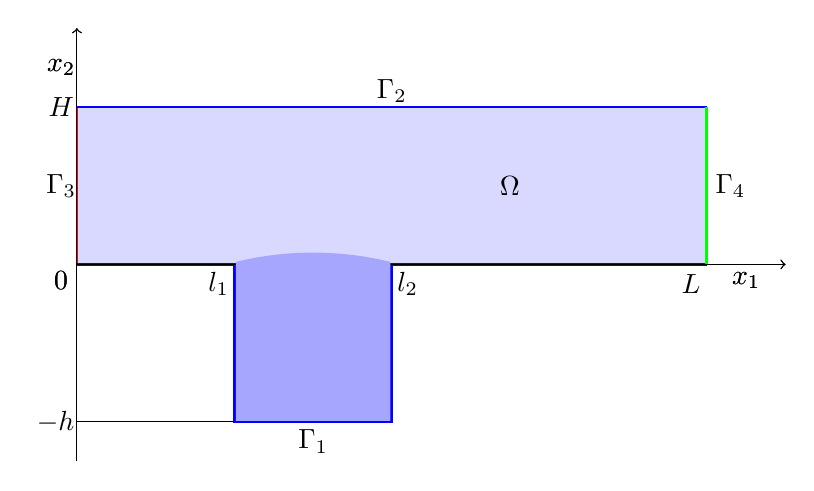
\begin{tikzpicture}
 	
 
   \fill [blue!15] (0,0) rectangle +(8.,4.);   
   \fill [white] (0,0) rectangle +(2.,2.);   
   \fill [white] (4,0) rectangle +(4.,2.);   

   
   
   \draw[->] (0,2) -- (9,2);
   \draw[->] (0,-0.5) -- (0,5);
   \draw(-0.2,2-0.2) node {$0$};   
   \draw(8.5,2-0.2) node {$x_1$};   
   \draw(-0.2,4.5) node {$x_2$};     
   \draw(-0.27,0) node {$-h$};
   \draw(-0.2,4) node {$H$}; 
   
   \draw[color=red,line width=1pt] (0,2) -- (0,4);
   \draw[color=blue,line width=1pt] (0,2) -- (2,2) -- (2,0) -- (4,0) -- (4,2) -- (8,2)  (0,4) -- (8,4);
   \draw[color=green,line width=1pt] (8,4)-- (8,2);
   \draw[-] (0,0) -- (2,0); 
 
   \draw(5.5,3) node {$\Omega$};
   \draw(2-0.2,2-0.25) node {$l_1$};   
   \draw(4+0.2,2-0.25) node {$l_2$};      
   \draw(8-0.2,2-0.25) node {$L$};   

   \draw(-0.2,3) node {$\Gamma_3$};
   \draw(8.3,3) node {$\Gamma_4$};
   \draw(4.,4.2) node {$\Gamma_2$};
   \draw(3.,-0.25) node {$\Gamma_1$};

 \draw[->] (0,2) -- (9,2);
\draw[->] (0,0) -- (0,5);
\draw(-0.2,2-0.2) node {$0$};   
\draw(8.5,2-0.2) node {$x_1$};   
\draw(-0.2,4.5) node {$x_2$};      

\clip (2.018,0.02) rectangle +(2-0.036,2.5);
{
\fill [blue!35] (3,0) ellipse (3 and 2.15);
%\draw[thick, purple] (1,0) ellipse (4 and 2.25);
}


 \end{tikzpicture}
\end{figure}


\end{document}

После: convert pdf to png
https://convertio.co/pdf-png/



 






